% Dokumentklassen s�ttes til memoir.
% Manual: http://ctan.org/tex-archive/macros/latex/contrib/memoir/memman.pdf
\documentclass[a4paper,oneside,article]{memoir}

\usepackage{pgf}
\usepackage{tikz}
\usepackage{pgfplots}
\usetikzlibrary{arrows,automata}
\usepackage{verbatim}
 
% Danske udtryk (fx figur og tabel) samt dansk orddeling og fonte med
% danske tegn. Hvis LaTeX brokker sig over �, � og � skal du udskifte
% "utf8" med "latin1" eller "applemac". 
\usepackage{inputenc}
\usepackage[danish]{babel}
\usepackage[T1]{fontenc}
 
% Matematisk udtryk, fede symboler, theoremer og fancy ting (fx k�debr�ker)
\usepackage{amsmath,amssymb}
\usepackage{bm}
\usepackage{amsthm}
%\usepackage{mathtools}
 
% Kodelisting. Husk at l�se manualen hvis du vil lave fancy ting.
% Manual: http://mirror.ctan.org/macros/latex/contrib/listings/listings.pdf
\usepackage{listings}
 
% Fancy ting med enheder og datatabeller. L�s manualen til pakken
% Manual: http://www.ctan.org/tex-archive/macros/latex/contrib/siunitx/siunitx.pdf
%\usepackage{siunitx}
 
% Inds�ttelse af grafik.
\usepackage{graphicx}
\usepackage{float}
 
% Reaktionsskemaer. L�s manualen for at se eksempler.
% Manual: http://www.ctan.org/tex-archive/macros/latex/contrib/mhchem/mhchem.pdf
%\usepackage[version=3]{mhchem}
%\usepackage[noend]{algpseudocode}
%\usepackage{algorithm}

\usepackage{xcolor,colortbl}

\usepackage{listings}

\definecolor{javared}{rgb}{0.6,0,0} % for strings
\definecolor{javagreen}{rgb}{0.25,0.5,0.35} % comments
\definecolor{javapurple}{rgb}{0.5,0,0.35} % keywords
\definecolor{javadocblue}{rgb}{0.25,0.35,0.75} % javadoc

\lstset{language=Java,
basicstyle=\small, %\ttfamily,
keywordstyle=\color{javapurple}\bfseries,
stringstyle=\color{javared},
commentstyle=\color{javagreen},
morecomment=[s][\color{javadocblue}]{/**}{*/},
numbers=left,
numberstyle=\tiny\color{black},
stepnumber=1,
numbersep=10pt,
tabsize=4,
showspaces=false,
showstringspaces=false}

\begin{document}
    \title{Remote Procedure Calls - Disposition}
    \author{Lukas Peter J�rgensen, 201206057, DA4
            }
    \maketitle
    
    RMI = RPC except that RMI operates on object instead of applications.
    \chapter{RPC}
	    \section{Difference between before and now}
	    	\begin{itemize}
		    	\item Transparent.
		    	\item Looks like normal procedure calls.
		    	\item Doesn't have to build directly over the internet primitives.
	    	\end{itemize}
	    \section{Sequence}
		    \begin{enumerate}
			    \item Client calls \textbf{client-stub}.
			    \item \textbf{Client stub} packs parameters into a message and makes a system call to send the message. (Packing is called marshalling).
			    \item Client OS sends the message.
			    \item Server OS passes the incoming message to the  \textbf{server-stub}
			    \item \textbf{Server stub} unpacks the parameters. (Unpacking is called unmarshalling).
			    \item \textbf{Server stub} the server procedure
		    \end{enumerate}
	\chapter{Marshalling}
	Example, 32-bit Intel to 32-bit SPARC (each field represents 1 byte (8 bits)).
	\begin{figure}[H]
	\centering
	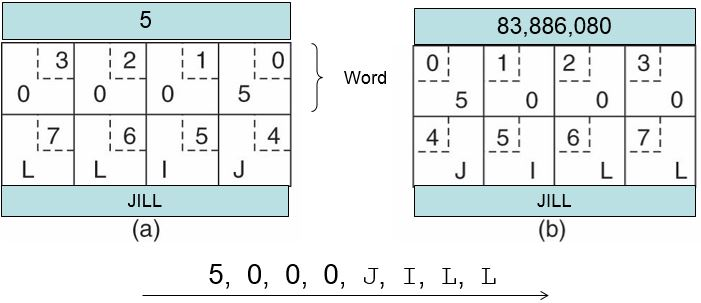
\includegraphics[width=\textwidth]{Media/MarshProb.jpg}
	\end{figure}
	
    \chapter{Synkron vs Asynkron}
   	\begin{figure}[H]
   	\centering
   	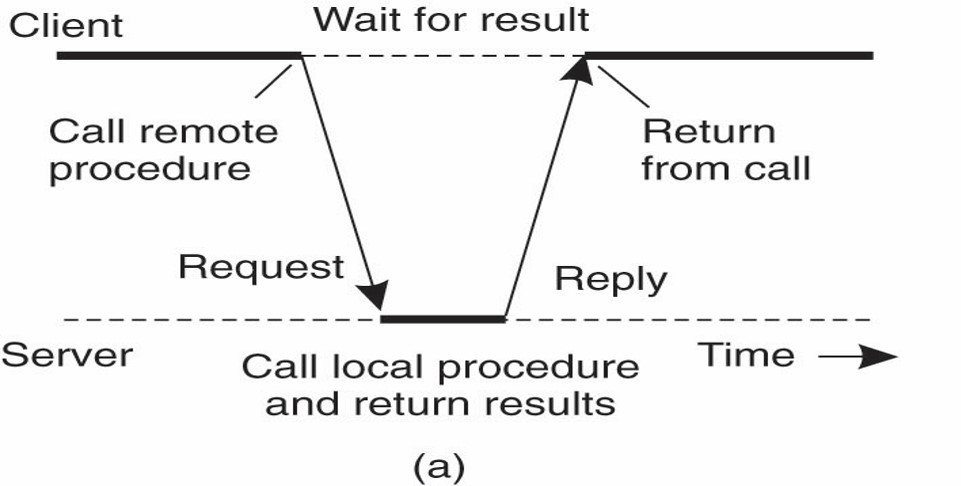
\includegraphics[width=\textwidth]{Media/SynchRPC.jpg}
   	\end{figure}
   	\section{Callback style}
	\begin{figure}[H]
	\centering
	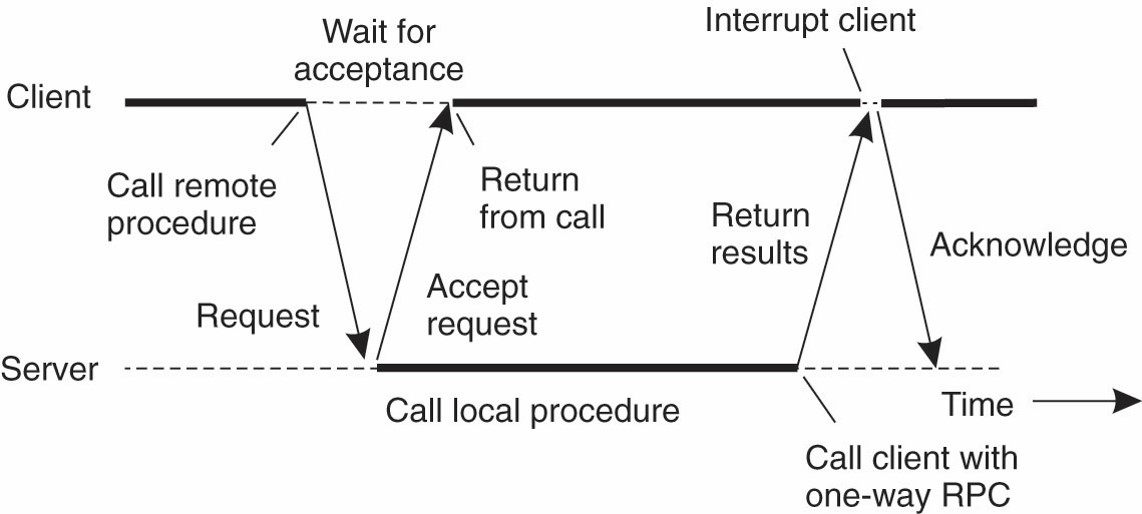
\includegraphics[width=\textwidth]{Media/ASynchRPC.jpg}
	\end{figure}
    
    
\end{document}